\chapter{General Description}
\label{chap:gendesc}
In this chapter we discuss the relation of this project to the ``outside world'': if there are any related projects running currently and if there were related projects in the past. Then, the purpose of the \applicationname{} and the environment in which it operates are discussed. After that, its relation to other systems is covered.

\section{Relation to current projects}
\label{sec:curproj}
%The context of this project in relation to other current projects
No other current projects are related to \projectname{}.

\section{Relation to predecessor and successor projects}
\label{sec:predsuc}
%The context of this project in relation to past and future projects
\projectname{} has multiple predecessor projects. These projects resulted in multiple Matlab\footnote{\url{http://www.mathworks.nl/products/matlab/}} tools that are available on the client's web page \cite{clientpage}. \projectname{} will combine some of the functionality of these tools into a mobile web application. \projectname{} will be developed in such a way that the client can easily extend the application with new mixers. When the development of \projectname{} is complete, the client will be responsible for maintaining the application. The client may change, add or remove the application's functionality. Finally, some general constraints are described and a description of the logical model is given.

\section{Function and purpose}
\label{sec:functpurp}
%A general overview of the function and purpose of the product
\projectname{} is an application that serves as an education tool for anyone who wants to gain a deeper understanding of the process of mixing in general, and in particular for students at the TU/e. By `playing' with the application, users can quickly and easily find out what the effects of a certain mixer and mixing protocol on an initial distribution are. This leads to a better understanding of the user about the way this mixer functions. \projectname{} may also be used as a quick and convenient way to observe whether a recently thought of mixing protocol renders good or bad mixing results. 

\section{Environment}
\label{sec:env}
%Hardware and operating system of target system and development system
\projectname{} is a web application that is developed primarily for use on mobile devices. This means the application will mostly be accessed through web browsers on smartphones and tablets. It is expected that the application will mostly be used on iPhones and iPads. Therefore, \projectname{} must support iOS Safari version 6.0 and above. Furthermore, \projectname{} should support Firefox versions 20 and above, and Google Chrome versions 26 and above. Lastly, if time permits, \projectname{} could also support Internet Explorer versions 10 and above, Opera versions 12.1 and above, and Safari versions 6.0 and above. \\
Since it is expected that the application will mostly be used on iPhones and iPads, the \applicationname must run on devices running on iOS versions 6 and higher. Furthermore, since a significant share of smartphones and tablets run on Android, \projectname{} should run on devices running on Android versions 4.0 and higher. Lastly, if time permits, \projectname{} could also run on devices running on Windows 8.\\
The hardware used by the users must be able to run at least one of the supported operating systems and browsers.\\
\todo{Moeten we hier nog iets zeggen over de screensize/resolution van de smartphones? Ik kan me voorstellen dat de applicatie niet prettig zal werken op zeer kleine schermen...}

\section{Relation to other systems}
\label{sec:othersys}
\todo{Is the product an independent system, part of a larger system, replacing another system? The essential characteristics of these other systems}

\section{General constraints}
\label{sec:genconst}
\todo{Reasons why constraints exist: background information and justification(analogous to URD)}

\section{Model description}
On a very high level, the architecture of \applicationname can be divided into different tiers communicating through communication channels. A graphical representation of these relation between those tiers and channels can be found in figure \ref{fig:tierchannel}.

\label{sec:moddesc}
\begin{figure}[h]
\label{fig:tierchannel}
  \centering
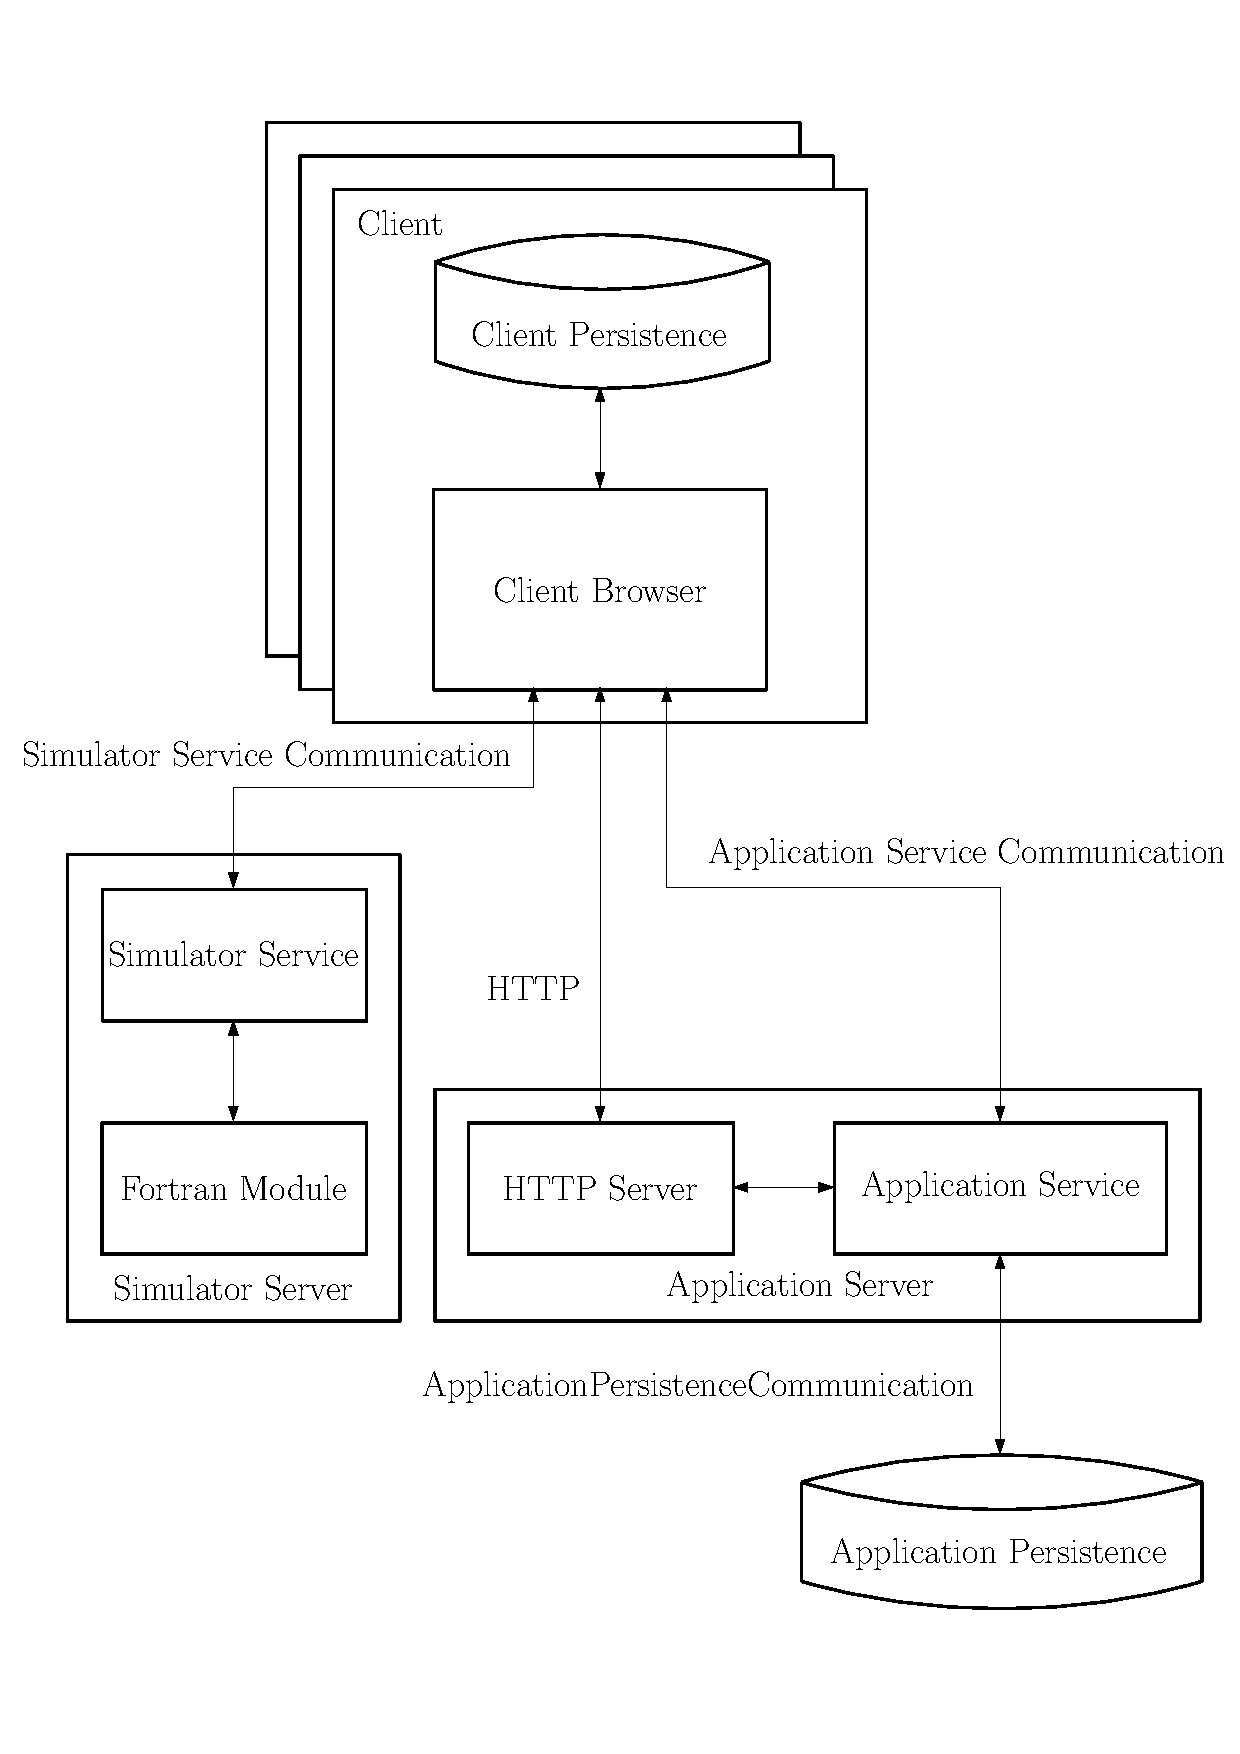
\includegraphics[scale=0.5]{SoftwareTiers}
\caption{The different tiers of the system}
\end{figure}